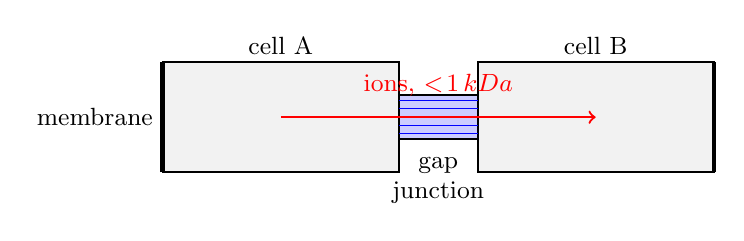
\begin{tikzpicture}[x=1.0cm, y=0.7cm, font=\small,
    every node/.style={align=left}]
  % Cell A
  \draw[thick,fill=gray!10] (0,0) rectangle (3,2);
  \node at (1.5,2.3) {cell A};
  % Cell B
  \draw[thick,fill=gray!10] (4,0) rectangle (7,2);
  \node at (5.5,2.3) {cell B};
  % Gap junction
  \draw[thick,fill=blue!20] (3,0.6) rectangle (4,1.4);
  \node[below] at (3.5,0.45) {gap};
  \node[below] at (3.5,0) {junction};
  % Connexin hexamer schematic
  \foreach \y in {0.7,0.85,1.0,1.15,1.3}{
    \draw[blue] (3,\y) -- (4,\y);
  }
  % Ion passage arrows
  \draw[->,thick,red] (1.5,1.0) -- (5.5,1.0);
  \node[red,above] at (3.5,1.2) {ions, $<\!1\,\text{kDa}$};
  % Membrane lines
  \draw[ultra thick] (0,0) -- (0,2);
  \draw[ultra thick] (7,0) -- (7,2);
  \node[left] at (0,1) {membrane};
\end{tikzpicture}
